\documentclass[a4paper, 10pt]{article}
\usepackage{scrextend}
\changefontsizes{9pt}
% Per-subject config for this repo. See vendor/template/course-config.tex.example
% for what each macro is used for.

\newcommand{\CourseCode}{2110473}
\newcommand{\CourseName}{Fault Tolerant Computing}
\newcommand{\StudentID}{6733172621}
\newcommand{\StudentName}{Patthadon Phengpinij}
\newcommand{\DefaultCollaborators}{Claude (for\,\LaTeX\,styling and grammar checking)}
\newcommand{\AssignmentLabel}{Homework}

\usepackage{../vendor/template/CEDT-Assignment-style}

\begin{document}
\subject
\asgntitle{9}{}{Week 11}{\StudentID\ \StudentName}{\DefaultCollaborators}

% ================================================================================ %
\section{Delay Fault Testing}
% ================================================================================ %

From the circuit below, Find Delay Fault Test Input Vector in case of

\begin{center}
	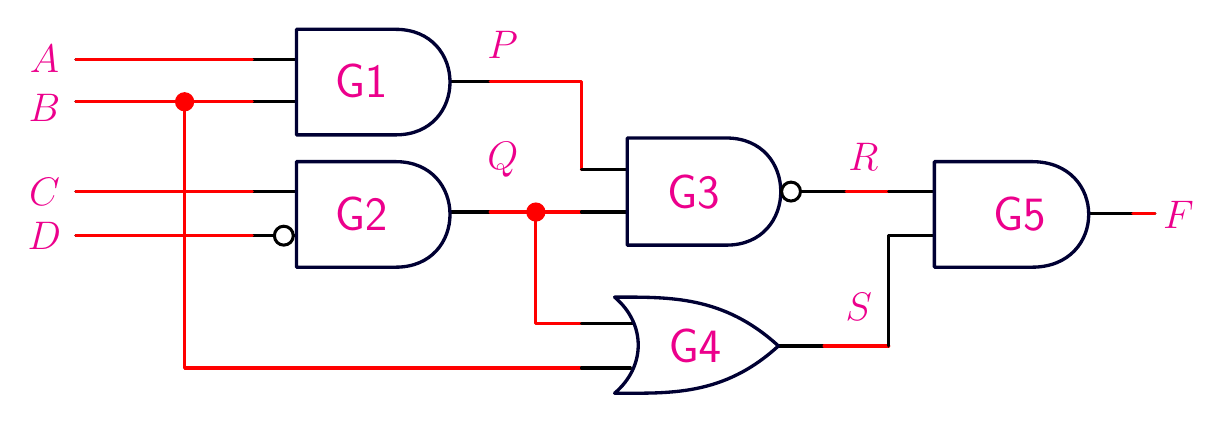
\begin{tikzpicture}[
			x=0.020cm, y=-0.020cm,
			wire/.style={
					draw=black,
					line width=1.15pt,
					line cap=round,
					line join=round
				},
			active/.style={
					draw=red,
					line width=1.15pt,
					line cap=round,
					line join=round
				},
			gate/.style={
					draw=blue!20!black,
					fill=white,
					line width=1.2pt,
					line join=round
				},
			dot/.style={
					circle,
					fill=red,
					draw=red,
					inner sep=0pt,
					minimum size=0.23cm
				},
			sig/.style={
					font=\Large,
					text=magenta,
					inner sep=0pt
				},
			gtext/.style={
					font=\sffamily\LARGE,
					text=magenta,
					inner sep=0pt
				},
			bubble/.style={
					draw=black,
					fill=white,
					line width=1.1pt
				}
		]

		% =========================================================
		% Input wires
		% =========================================================

		% Input A
		\draw[wire] (53,38) -- (193,38);
		\draw[active] (53,38) -- (165,38);

		% Input B
		\draw[wire] (53,65) -- (193,65);
		\draw[active] (53,65) -- (165,65);

		% Input C
		\draw[wire] (53,122) -- (193,122);
		\draw[active] (53,122) -- (165,122);

		% Input D (inverted)
		\draw[wire] (53,150) -- (179,150);
		\draw[active] (53,150) -- (165,150);
		\draw[wire] (191,150) -- (193,150);

		% =========================================================
		% Branch from B to G4
		% =========================================================

		\draw[active]
		(122,65) -- (122,234) -- (374,234);

		\draw[wire]
		(374,234) -- (405,234);

		% =========================================================
		% G1 output P -> G3
		% =========================================================

		\draw[wire]
		(291,52) -- (316,52);

		\draw[active]
		(316,52) -- (374,52) -- (374,108);

		\draw[wire]
		(374,108) -- (403,108);

		% =========================================================
		% G2 output Q -> G3 and G4
		% =========================================================

		\draw[wire]
		(291,135) -- (316,135);

		\draw[active]
		(316,135) -- (374,135);

		\draw[wire]
		(374,135) -- (403,135);

		% Q branch to G4
		\draw[active]
		(345,135) -- (345,206) -- (374,206);

		\draw[wire]
		(374,206) -- (407,206);

		% =========================================================
		% G3 output R -> G5
		% =========================================================

		% NAND output and R wire
		\draw[wire]
		(513,122) -- (542,122);

		\draw[active]
		(542,122) -- (569,122);

		\draw[wire]
		(569,122) -- (598,122);

		% =========================================================
		% G4 output S -> G5
		% =========================================================

		\draw[wire]
		(499,220) -- (528,220);

		\draw[active]
		(528,220) -- (569,220);

		\draw[wire]
		(569,220) -- (569,150) -- (598,150);

		% =========================================================
		% G5 output F
		% =========================================================

		\draw[wire]
		(695,136) -- (738,136);

		\draw[active]
		(724,136) -- (738,136);

		% =========================================================
		% G1 : AND gate
		% =========================================================

		\draw[gate]
		(193,19) -- (256,19)
		.. controls (302,19) and (302,86) .. (256,86)
		-- (193,86) -- cycle;

		% =========================================================
		% G2 : AND gate
		% =========================================================

		\draw[gate]
		(193,103) -- (256,103)
		.. controls (302,103) and (302,170) .. (256,170)
		-- (193,170) -- cycle;

		% =========================================================
		% G3 : NAND gate
		% =========================================================

		\draw[gate]
		(403,88) -- (466,88)
		.. controls (512,88) and (512,156) .. (466,156)
		-- (403,156) -- cycle;

		% NAND inversion bubble
		\draw[bubble]
		(507,122) circle[radius=6];

		% =========================================================
		% G4 : OR gate
		% =========================================================

		\draw[gate]
		(395,189)
		.. controls (430,189) and (464,188) .. (499,220)
		.. controls (464,252) and (430,250) .. (395,250)
		.. controls (415,233) and (415,206) .. (395,189)
		-- cycle;

		% =========================================================
		% G5 : AND gate
		% =========================================================

		\draw[gate]
		(598,103) -- (660,103)
		.. controls (708,103) and (708,170) .. (660,170)
		-- (598,170) -- cycle;

		% =========================================================
		% D input inversion bubble
		% =========================================================

		\draw[bubble]
		(185,150) circle[radius=6];

		% =========================================================
		% Junction dots
		% =========================================================

		\node[dot] at (122,65) {};
		\node[dot] at (345,135) {};

		% =========================================================
		% Gate labels
		% =========================================================

		\node[gtext] at (234,52)  {G1};
		\node[gtext] at (234,136) {G2};
		\node[gtext] at (445,122) {G3};
		\node[gtext] at (446,220) {G4};
		\node[gtext] at (652,136) {G5};

		% =========================================================
		% Input labels
		% =========================================================

		\node[sig] at (33,38)  {$A$};
		\node[sig] at (33,69)  {$B$};
		\node[sig] at (33,122) {$C$};
		\node[sig] at (33,150) {$D$};

		% =========================================================
		% Intermediate signal labels
		% =========================================================

		\node[sig] at (324,29)  {$P$};
		\node[sig] at (324,102) {$Q$};
		\node[sig] at (553,100) {$R$};
		\node[sig] at (550,195) {$S$};

		% =========================================================
		% Output label
		% =========================================================

		\node[sig] at (753,137) {$F$};

	\end{tikzpicture}
\end{center}

\noindent Circuit functions (used in both problems):
\begin{align*}
	P & = AB, \qquad Q = C\overline{D}, \qquad R = \overline{PQ}, \qquad S = Q + B,   \\
	F & = R\cdot S = \overline{AB\,C\overline{D}}\cdot\left(C\overline{D} + B\right).
\end{align*}
A delay fault test is a vector pair \( \langle V_1, V_2 \rangle \) (written as \( ABCD \)):
\( V_1 \) initializes the path, \( V_2 \) launches the transition. To sensitize a path, every
side input must be held \emph{stable} at the non-controlling value of its gate
(1 for AND/NAND, 0 for OR) in both vectors, so that the output transition depends only on the
transition travelling along the path (robust test).

% ================================================================================ %
%                                    Problem 01                                    %
% ================================================================================ %
\begin{problem}
\( \downarrow A \) transition
\end{problem}

\begin{solution}
	\noindent Path: \( A \to P\,(G1) \to R\,(G3) \to F\,(G5) \).
	\begin{itemize}
		\item \textbf{G1 (AND):} side input \( B = 1 \).
		\item \textbf{G3 (NAND):} side input \( Q = C\overline{D} = 1 \Rightarrow C = 1,\ D = 0 \).
		\item \textbf{G5 (AND):} side input \( S = Q + B = 1 \) (already satisfied, and stable since \( Q = 1 \)).
	\end{itemize}
	\begin{center}
		\begin{tabular}{c|cccc|cccc|c}
			\toprule
			          & \( A \)          & \( B \) & \( C \) & \( D \) & \( P \)          & \( Q \) & \( R \)        & \( S \) & \( F \)        \\
			\midrule
			\( V_1 \) & 1                & 1       & 1       & 0       & 1                & 1       & 0              & 1       & 0              \\
			\( V_2 \) & 0                & 1       & 1       & 0       & 0                & 1       & 1              & 1       & 1              \\
			\midrule
			          & \( \downarrow \) & 1       & 1       & 0       & \( \downarrow \) & 1       & \( \uparrow \) & 1       & \( \uparrow \) \\
			\bottomrule
		\end{tabular}
	\end{center}
	\[ \boxed{\langle V_1, V_2 \rangle = \langle ABCD = 1110,\ ABCD = 0110 \rangle} \]
	The \( \downarrow A \) transition appears at the output as \( \uparrow F \) (inverted once by the NAND).
	If \( F \) is sampled before it has risen to 1, the path \( A\text{-}P\text{-}R\text{-}F \) has a delay fault.
	This test is unique, since \( B, C, D \) are all forced.
\end{solution}
% ================================================================================ %

\newpage

% ================================================================================ %
%                                    Problem 02                                    %
% ================================================================================ %
\begin{problem}
\( \uparrow B \) transition
\end{problem}

\begin{solution}
	\noindent \( B \) fans out to two paths that reconverge at G5, so each path needs its own test:
	\begin{center}
		Path 1: \( B \to P\,(G1) \to R\,(G3) \to F\,(G5) \), \qquad
		Path 2: \( B \to S\,(G4) \to F\,(G5) \).
	\end{center}

	\noindent\textbf{Path 1} \( (B\text{-}P\text{-}R\text{-}F) \):
	\begin{itemize}
		\item \textbf{G1 (AND):} \( A = 1 \).
		\item \textbf{G3 (NAND):} \( Q = 1 \Rightarrow C = 1,\ D = 0 \).
		\item \textbf{G5 (AND):} \( S = Q + B = 1 \), stable because \( Q = 1 \) holds \( S \) at 1 while \( B \) changes.
	\end{itemize}
	\begin{center}
		\begin{tabular}{c|cccc|cccc|c}
			\toprule
			          & \( A \) & \( B \)        & \( C \) & \( D \) & \( P \)        & \( Q \) & \( R \)          & \( S \) & \( F \)          \\
			\midrule
			\( V_1 \) & 1       & 0              & 1       & 0       & 0              & 1       & 1                & 1       & 1                \\
			\( V_2 \) & 1       & 1              & 1       & 0       & 1              & 1       & 0                & 1       & 0                \\
			\midrule
			          & 1       & \( \uparrow \) & 1       & 0       & \( \uparrow \) & 1       & \( \downarrow \) & 1       & \( \downarrow \) \\
			\bottomrule
		\end{tabular}
	\end{center}
	\[ \boxed{\text{Path 1: } \langle V_1, V_2 \rangle = \langle 1010,\ 1110 \rangle} \quad (\uparrow B \Rightarrow\ \downarrow F) \]

	\noindent\textbf{Path 2} \( (B\text{-}S\text{-}F) \):
	\begin{itemize}
		\item \textbf{G4 (OR):} \( Q = C\overline{D} = 0 \Rightarrow (C, D) \neq (1, 0) \).
		\item \textbf{G5 (AND):} \( R = \overline{PQ} = 1 \), which holds automatically (and stays stable) because \( Q = 0 \).
		\item \( A \) is a don't-care; choose \( A = 0 \), \( C = D = 0 \).
	\end{itemize}
	\begin{center}
		\begin{tabular}{c|cccc|cccc|c}
			\toprule
			          & \( A \) & \( B \)        & \( C \) & \( D \) & \( P \) & \( Q \) & \( R \) & \( S \)        & \( F \)        \\
			\midrule
			\( V_1 \) & 0       & 0              & 0       & 0       & 0       & 0       & 1       & 0              & 0              \\
			\( V_2 \) & 0       & 1              & 0       & 0       & 0       & 0       & 1       & 1              & 1              \\
			\midrule
			          & 0       & \( \uparrow \) & 0       & 0       & 0       & 0       & 1       & \( \uparrow \) & \( \uparrow \) \\
			\bottomrule
		\end{tabular}
	\end{center}
	\[ \boxed{\text{Path 2: } \langle V_1, V_2 \rangle = \langle 0000,\ 0100 \rangle} \quad (\uparrow B \Rightarrow\ \uparrow F) \]
	(Any \( A \in \{0,1\} \) with \( CD \in \{00, 01, 11\} \) also works, e.g.\ \( \langle 1001, 1101 \rangle \).)

	\medskip
	\noindent The two paths cannot be tested by one vector pair: Path 1 requires \( Q = 1 \)
	while Path 2 requires \( Q = 0 \). Hence both pairs are needed to cover \( \uparrow B \).
\end{solution}
% ================================================================================ %

\end{document}
